\documentclass{article}
\usepackage{times}
\usepackage{natbib}[round]
\usepackage[titletoc]{appendix}
\usepackage{graphicx}
\usepackage{lineno}
\usepackage{multirow}
\usepackage[english]{babel}
\usepackage{typearea} 
\usepackage{amssymb}
\usepackage{amsfonts}
\usepackage{amsmath}
\usepackage{enumerate}
\usepackage{mathtools}
\usepackage{graphicx}
\usepackage{wrapfig}
\usepackage{lscape}
\usepackage{rotating}
\newcommand{\Fig}[1]{Figure~\ref{fig:#1}}

\renewcommand{\baselinestretch}{1.5}
\newcommand{\bbar}[1]{\overline{#1}}

\newcommand\scalemath[2]{\scalebox{#1}{\mbox{\ensuremath{\displaystyle #2}}}}
\renewcommand{\familydefault}{\sfdefault}

\usepackage[font={small},labelfont={bf},justification=justified,margin=0.5cm]{caption}

\renewcommand{\thesection}{}
\renewcommand{\thesubsection}{\arabic{section}.\arabic{subsection}}

\usepackage{color}
	 \definecolor{darkred}{rgb}{0.75,0,0}
%	 \definecolor{darkgreen}{rgb}{0,0.5,0}
	 \definecolor{darkblue}{rgb}{0,0,0.75}
%	 \definecolor{magenta}{rgb}{0,0,0.75}
\newcommand{\cha}[1]{\textcolor{darkblue}{(#1)}}
\newcommand{\phg}[1]{\textcolor{darkred}{(#1)}}


\usepackage{hyperref}
\definecolor{darkgreen}{rgb}{0.1,0.6,0.3}
\definecolor{darkred}{rgb}{0.6,0.3,0.1}
\hypersetup{
    colorlinks=true,       % false: boxed links; true: colored links
    linkcolor=blue,          % color of internal links (change box color with linkbordercolor)
    citecolor=darkgreen,        % color of links to bibliography
    filecolor=magenta,      % color of file links
    urlcolor= black           % color of external links
}


\title{\vspace*{-22mm}\bf Multiple infections and complex life cycles}
%\author{Vaibhvi$^{1}$,
%Chaitanya S. Gokhale$^{2*}$\\
%\normalsize $^1$Molecular Physiology Group, \\
%\normalsize University of Kiel, \\
%\normalsize Am Botanisch Garten 3-9, D-24118 Kiel, Germany.\\
%\normalsize $^2$Research Group for Theoretical Models of Eco-evolutionary Dynamics, \\
%\normalsize Department of Evolutionary Theory, Max Planck Institute for Evolutionary Biology, \\
%\normalsize August-Thienemann-Stra{\ss}e 2, 24306 Pl\"{o}n, Germany.\\
%\normalsize $^{*}$gokhale@evolbio.mpg.de
%}

\date{}

\begin{document}

\linenumbers
\maketitle


\begin{abstract}
Abstract
\end{abstract}


\noindent
Keywords: a,b,c,d


\tableofcontents

\section{Introduction}

Life on earth is ubiquitously infested with parasite, many with complex life cycles \citep{zimmer:book:2001}.
While a complex life cycle can be defined as abrupt ontogenic changes in morphology and/or ecology \citep{Benesh:2016dj}, a complex parasitic life cycle typically involves numerous hosts that a parasite needs to traverse in the process of completing its life cycle.
Helminths are a prime example of how a successive transmission between multiple host species is necessary for developing the next generation.
The worms occupy different niches (hosts) in different stages of their lifecycle, moving through intermediate hosts until reaching a definitive host in which reproduction can finally occur.
Numerous factors determine the transmissibility and infectivity of the parasites along the tropic level of hosts \citep{froelick:PRSB:2021}.
Comparative growth rate, eventual body size, cost-benefits of host-manipulation and the probability of eventually finding a mate all play a major role in the development and maintenance of the life-history strategies of such parasites \citep{parker:Nature:2003,hammerschmidt:Evolution:2009} \cha{more references?}.
An integral part of all the above factors is the comparative approach.
Parasite often co-occur in the same host and this allows for complex within-host interactions since the evolutionary effect of the actions is not realised till reproduction occurs in the definitive host \citep{Hafer:2015gl}.

\cha{Discuss the work by \citep{alizon:AmNat:2008,gandon:Evolution:2009} 
What is done in those studies and what is the gap that exists. How do we fill in exactly that gap!}


In this manuscript we focus on dissecting the fundamental trade-off between transmissibility and host-manipulation when multiple hosts are present in a host and its evolutionary outcome in the associated trait space.

\section{Model}
We focus on the complex lifecycle of a trophically transmitted parasite. 
Parasites reproduce inside their definitive hosts and are released into the environment. 
They infect intermediate hosts when the hosts encounter the parasite pool. 
When an infected intermediate host is consumed by a definitive host, the definitive host gets infected and the parasite complete its lifecycle.

For simplicity, intermediate and definitive hosts can be infected by one (single infection) or at most two parasites (double infections). 
Therefore, $p$ is the probability that two parasites in the parasite pool co-transmit to an intermediate host, and $1-p$ is the probability that a single parasites enters an intermediate host. 
When a definitive host consumes an intermediate host infected by two parasites, there is a probability $q$ that both parasites co-transmit to the definitive host, and $1-q$ is the probability that only one parasite successfully transmits. 
The dynamics of a complex lifecycle parasite that requires two hosts is described by the following ODEs, firstly for the intermediate host as,

\begin{align}
\frac{dI_s}{dt} &= R(I_s, I_w, I_{ww}) - d I_s - \Pi_s(D_s, D_w, D_{ww}) I_s  - \eta_w  I_s \nonumber \\ 
\frac{dI_w}{dt} &=  (1 - p) \eta_w I_s  - (d + \alpha_w) I_w - \Pi_w(D_s, D_w, D_{ww}, \beta_w) I_w \label{odes:ihosts} \\
\frac{dI_{ww}}{dt} &= p \eta_w I_s  - (d + \alpha_ww) I_{ww} - \Pi_{ww}(D_s, D_w, D_{ww}, \beta_{ww}) I_{ww} \nonumber
\end{align}

where  $R(I_s, I_w, I_{ww})$ represents the birth rate of the intermediate hosts, which is a function of both infected and noninfected individuals. 
In other words, all types of intermediate hosts can reproduce. 
$\Pi_i$, where $i = \{s, w, ww\}$ is the predation function of definitive hosts on respectively, susceptible, singly infected and doubly infected intermediate hosts. 
The predation function depends on the density of the definitive hosts and the manipulative strategies of parasites in the intermediate hosts. 
In particular, if an intermediate host is infected by a single parasite, the manipulation strategy is $\beta_w$, and if it is infected by two parasites, the manipulation strategy is $\beta_{ww}$. 
There is a link between $\beta_w$ and $\beta_{ww}$, but we need not specify the link for now. 
$\eta_w = \gamma W$ is the force of infection by parasites in the environment. 
$\lambda_i = \beta_i I_i$, where $i = \{ w, ww\}$, is the force of infection that corresponds respectively to singly infected intermediate host ($I_w$), or doubly infected intermediate hosts ($I_{ww}$). 

For the definitive hosts we have,
\begin{align}
\frac{dD_s}{dt} &= B(D_s,  D_w,  D_{ww},  I_s, I_w, I_{ww})  - \mu D_s - (\lambda_{ww} + \lambda_w) D_s \nonumber \\    
\frac{dD_w}{dt} &= (\lambda_w + (1 - q) \lambda_{ww}) D_s - (\mu + \sigma_w) Dw - ((1 - q) \lambda_{ww} + \lambda_w) D_w  \label{odes:dhosts} \\         
\frac{dD_{ww}}{dt} &= q \lambda_{ww} D_s + ((1 - q) \lambda_{ww} + \lambda_w) D_w - (\mu + \sigma_{ww}) D_{ww} \nonumber
\end{align}
%
where $B(D_s, D_w, D_{ww}, I_s, I_w, I_{ww})$ represents the birth rate of definitive hosts, which is a function of population density of both intermediate and definitive hosts, infected or non-infected alike. 
The dynamics of the parasites are then given solely by,
\begin{align}
	\frac{dW}{dt} &= f_w D_w + f_{ww} D_{ww} - \delta W - \eta_w I_s \label{odes:eparasite}
\end{align}


Definitions of different parameters can be found in Table \ref{table:varpardescription}.

\begin{table}[!ht]
\begin{tabular}{|p{2.5cm}|p{12cm}|} 
\hline
Parameters and Variables    &  Description  \\
\hline
$I_i$  & Density of intermediate hosts that are susceptible $i=s$, singly infected $i=w$, or doubly infected $i=ww$ \\
\hline
$D_i$ & Density of definitive hosts that are susceptible $i=s$, singly infected $i=w$, or doubly infected $i=ww$ \\
\hline
$W$ & Density of parasites released from definitive hosts into the environment \\
\hline
$d$ & Natural death rate of intermediate hosts \\
\hline
$\alpha_i$ & Additional death rate of intermediate hosts due to infection by a single parasite ($i = w$) or two parasites ($i = ww$) \\
\hline
$p$ & Probability that two parasites cotransmit from the environment to an intermediate host \\
\hline
$\gamma$ & Transmission rate of parasites in the environment to intermediate hosts \\
\hline
$\mu$ & Natural death rate of definitive hosts \\
\hline
$\sigma_i$ & Additional death rate of definitive hosts due to infection by a single parasite ($i = w$) or two parasites ($i = ww$) \\
\hline
$\sigma_i$ & Additional death rate of the hosts due to being infected by a singly parasite ($i = w$) or two parasites ($i = ww$) \\
\hline
$q$ & Probability that two parasites cotransmit from intermediate hosts to definitive hosts \\
\hline
$\beta_i$ & Transmission rate of parasites from intermediate hosts to definitive hosts \\
\hline
$f_i$ & Reproduction rate of parasites in singly infected definitive hosts ($i = w$) or doubly infected hosts ($i = ww$)\\
\hline
$\delta$ & Natural death rate of parasites in the environment \\
\hline
\end{tabular}
\caption{Description of variables and parameters}
\label{table:varpardescription}
\end{table}

For simplicity, we assume that there is no sequential infection when parasites transmit from the environment to intermediate hosts. 
Sequential infection can happen when parasites transmit from intermediate hosts to definitive hosts. 
Therefore, a singly infected definitive host can be further infected by another parasite if it consumes infected intermediate hosts. The dynamics of the system are illustrated in figure (\ref{fig:schematic}).

\begin{figure}
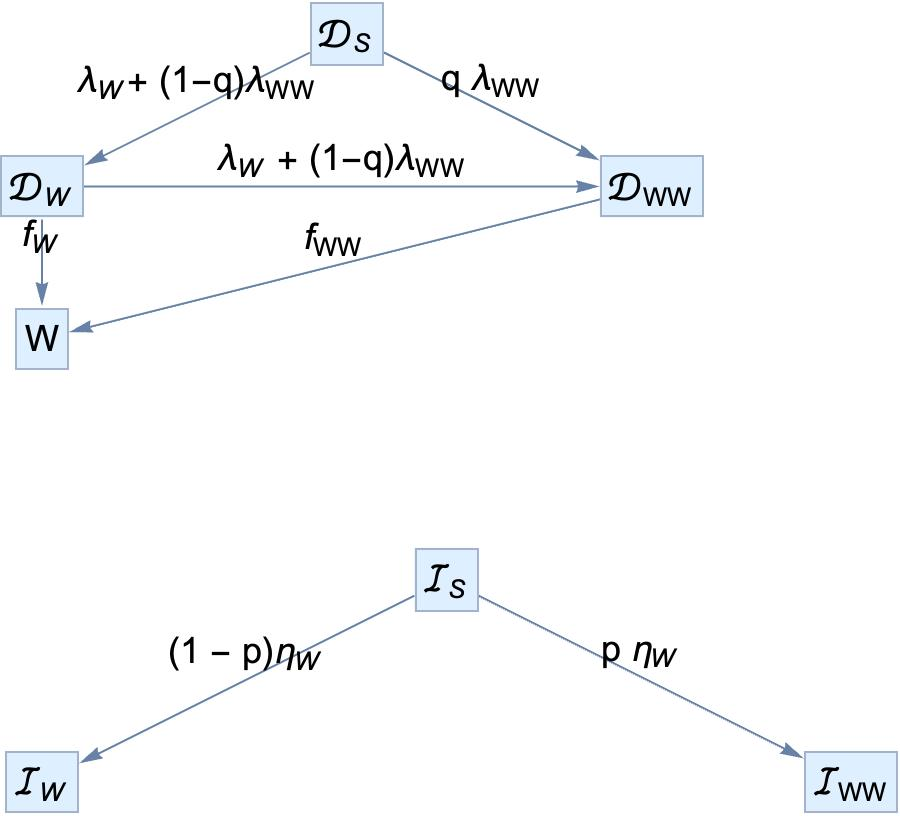
\includegraphics[width=\textwidth]{schematic}
\caption{Schematic of the model}
\label{fig:schematic}
\end{figure}

\subsection{Resident dynamics}

\phg{In this part, I just want to list what I understand about the dynamics, so not all of them will be in the ms}

System (\ref{odes:ihosts}, \ref{odes:dhosts}, \ref{odes:eparasite}) always has a parasite free state, that is the parasite population is zero or $W = I_w = I_ww = D_w = D_ww = 0$. In this disease-free state, if a parasite arises, the population can spread when its reproduction ratio $R_0$ in this disease-free state is greater than one. The expression of the $R_0$ is as followed

\begin{align}
R_{0res} = & \frac{f_{ww}}{\gamma  I_s + \delta } \frac{(1-p) \gamma}{\alpha_w + d + \Pi_w} I_s \frac{\beta_w (\lambda_w +  (1-q)\lambda_{ww})}{(\mu + \sigma_{ww}) (\lambda_w + \mu + (1-q) \lambda_{ww} + \sigma_w)} D_s + \nonumber \\ 
           & \frac{f_{ww}}{\gamma  I_s + \delta }  \frac{p \gamma}{\alpha_{ww} + d + \Pi_{ww}} I_s  \frac{(1-q) \beta_{ww} (\lambda_w +(1-q) \lambda_{ww})}{(\mu +\sigma_{ww}) (\lambda_w + (1-q) \lambda_{ww} + \mu + \sigma_w)} D_s + \nonumber \\
           & \frac{f_{ww}}{\gamma  I_s + \delta }  \frac{p \gamma}{\alpha_{ww} + d + \Pi_{ww}} I_s  \frac{q \beta_{ww}}{\mu +\sigma_{ww}} D_s  \\
           & \frac{f_w}{\gamma  I_s + \delta }  \frac{(1-p) \gamma}{\alpha_w + d + \Pi_w} I_s  \frac{\beta_w}{\lambda_w + (1-q)\lambda_{ww} +\mu + \sigma_w} D_s + \nonumber \\
           & \frac{f_w}{\gamma  I_s + \delta } (p \gamma)/(d + \alpha_{ww} + \Pi_{ww}) I_s \frac{(1-q) \beta_{ww}}{\lambda_w + (1-q) \lambda_{ww} + \mu +\ sigma_w} D_s \nonumber
\end{align}

$R_0$ of a parasite in the disease-free state is composed of different compartment reproduction ratios that correspond to different routes of infection that the parasite can follow. It should be noted that if a parasite is released from a doubly infected definitive host, it will always end up co-infected with another parasite. In contrast, if the parasite is released from a singly infected definitive host, it ends up in a singly infected host (\phg{we will need to understand why}).

When we introduce a parasite in the disease-free state, the parasite population can persist if its reproduction ratio $R_0|_{W = I_w = I_ww = D_w = D_ww = 0} > 1$. However, to solve this inequality, we need to specify the predation functions and the equilibrium value of $I_s$ and $D_s$. The explicit forms of the equilibrium of intermediate and definitive hosts depend largely on the birth functions $R$ and $B$ of respectively the intermediate and definitive host, and predation functions $\Pi_s, \Pi_w, \Pi_ww$. For simplicity, we consider linear functions for predation 
\begin{align*}
& \Pi_s = \rho (D_s + D_w + D_{ww}) \\
& \Pi_w(D_s, D_w, D_{ww}, \beta_w) = (\rho + \beta_w) (Ds + Dw + Dww) \\
& \Pi_{ww}(D_s, D_w, D_{ww}, \beta_{ww}) = (\rho + \beta_{ww}) (Ds + Dw + Dww)
\end{align*}
Here $\rho$ is the baseline capture rate when the uninfected intermediate hosts are caught by definitive hosts. Manipulation strategy of the parasite is incorporated as an addition to the baseline capture rate $\rho$. The birth function of definitive hosts is also linear
\begin{align*}
B(D_s, D_w, D_{ww}, I_s, I_w, I_{ww}) = \rho c (D_s + D_w + D_{ww}) (I_s + I_w + I_{ww})
\end{align*}
where c is the efficiency of converting preys into offspring.

\subsection{Linear birth function of intermediate hosts}
We consider the system when the birth function $R$ is linear, that is, $R(I_s, I_w, I_ww) = r(I_s + I_w + I_ww)$. The equilibrium of intermediate and definitive hosts in the disease-free state are

\begin{align*}
& I_{s0}^* = \frac{\mu}{c \rho} \\
& D_{s0}^* = \frac{r - d}{\rho}
\end{align*}

This equilibrium is always unstable. In fact, we always observe cyclic behaviour of the equilibrium because at this equilibrium the jacobian matrix of system (\ref{odes:ihosts}, \ref{odes:dhosts}, \ref{odes:eparasite}) always has one imaginary eigen value with positive real part. This is in accordance with the Lotka-Voltera system using linear functions for prey birth and predation. Because the disease-free dynamics is cyclic, it is difficult to analyse the spread of a parasite (which is often evaluate when the disease-free state is stable). Here, even if we solve the inequality $R_0 > 1$, which happens when the transmission rate from the environment to intermediate hosts $\gamma$ is greater than a threshold (the expression of the threshold is too complicated, hence it is not useful to write it here). In addition, the reproduction of the parasites has to be sufficiently large (again, the expression of the thresholds are too complicated such that it is useless to write it here).

In fact, our simulations show that the parasite cannot persist even when its reproduction ratio is greater than one. This result is, however, in agreement with the conclusion in \citet{Ripa:Evol:2013}, which suggests that it is harder for a mutant to invade a cyclic population. In our case, it is the invasion of a parasite in a cyclic disease-free host population.


We then consider the evolution of the host manipulation strategy $\beta_w$. Assuming that mutation is so rare, a mutant with a manipulation strategy $\beta_m$ that is slightly different from the resident arises when the resident parasite reaches its ecological equilibrium.

\subsection{Mutant dynamics}
Considering that a resident parasite with dynamics (\ref{odes:ihosts}, \ref{odes:dhosts}, \ref{odes:eparasite}) is at its non-zero equilibrium ($W^*, I_s^*, I_w^*, I_{ww}^*, D_s^*, D_w^*, D_{ww}^*$), the dynamics of a rare mutant parasite that enter the resident population will be

\begin{subequations}
\begin{align}
& \frac{dI_m}{dt} = (1 - p) \frac{M}{M + W^*} \eta I_s - (d + \alpha_m) I_m -\Pi_m(D_s^*, D_w^*,  D_{ww}^*,  \beta_m, D_m, D_{mm}, D_{mw}) I_m \\
& \frac{dI_{mm}}{dt} = p \frac{M^2}{(M + W^*)^2} \eta I_s - (d + \alpha_{mm}) I_{mm} - \Pi_{mm}(D_s^*, D_w^*, D_{ww}^*, \beta_{mm}, D_m, D_{mm}, D_{mw}) I_{mm}\\
& \frac{dI_{mw}}{dt} =  p \frac{2 M W^*}{(M + W^*)^2} \eta I_s - (d + \alpha_{mw}) I_{mw} -\Pi_{mw}(D_s^*, D_w^*, D_{ww}^*, \beta_{mw}, D_m, D_{mm}, D_{mw}) I_{mw} \\
& \frac{dD_m}{dt} = ( \lambda_m + (1 - q) (\lambda_{mm} + \lambda_{mw})) D_s - (\mu + \sigma_m) D_m - (\lambda_w + \lambda_m + (1 - q) (\lambda_{ww} + \lambda_{mw} + \lambda_{mm}) ) D_m \\
& \frac{dD_{mm}}{dt} = q \lambda_{mm} D_s + (\lambda_m + (1 - q)(\lambda_{mm} + \lambda_{mw})) D_m - (\mu + \sigma_{mm}) D_{mm} \\
& \frac{dD_{mw}}{dt} = q \lambda_{mw} D_s + (\lambda_m + (1 - q)(\lambda_{mm} + \lambda_{mw})) D_w + (\lambda_w + (1 - q) (\lambda_{ww} + \lambda_{mw})) D_m - (\mu + \sigma_{mw}) D_{mw} \\
& \frac{dM}{dt} = f_m D_m + f_{mm} D_{mm} +  f_{mw} D_{mw} - \delta M - \eta I_s;
\end{align}
\label{odes:mutdynamics}
\end{subequations}

where $\eta =\gamma (M + W^*)$ is the force of infection of parasites in the environment, which now includes both mutants and residents. $\lambda_m = \beta_m I_m$, $\lambda_{mm} = \beta_{mm} I_{mm}$, $\lambda_{mw} = \beta_{mw} I_{mw}$ are the force of infection of, respectively, intermediate hosts infected by a single mutant, two mutants, and a mix of mutant and resident. 

\subsection{Invasion fitness}
The invasion fitness of the mutant will be calculated using the next generation method \citep{hurford:JRSI:2010}.

The matrix $\mathbf{A}$ that describes the dynamics (\ref{odes:mutdynamics}) of the mutant can be written as $\mathbf{A} = \mathbf{F} - \mathbf{V}$, where $\mathbf{F}$ is the matrix that describes the contribution of a compartment to the next generation. Because we consider a complex lifecycle parasite, a new generation begins with the reproduction and release of parasites into the environment, and matrix $\mathbf{F}$ can be written as

\begin{align*}
    \mathbf{F} = 
    \begin{pmatrix}
   	 0 & 0 & 0 & 0   & 0 	  & 0 	   & 0 \\
	 0 & 0 & 0 & 0   & 0 	  & 0 	   & 0 \\
	 0 & 0 & 0 & 0   & 0 	  & 0 	   & 0 \\
	 0 & 0 & 0 & 0   & 0      & 0	   & 0 \\
	 0 & 0 & 0 & 0   & 0      & 0      & 0 \\ 
	 0 & 0 & 0 & 0   & 0      & 0      & 0 \\
	 0 & 0 & 0 & f_m & f_{mm} & f_{mw} & 0
    \end{pmatrix}
\end{align*}

The matrix $\mathbf{V}$ describes the transitions from one compartment to the others and death rates of all compartments
\[
    \mathbf{V} = 
    \begin{pmatrix*}
     v_{11}  & 0 & 0 & 0 & 0 & 0 & v_{17} \\
     0  &  v_{22} & 0 & 0 & 0 & 0 & v_{27} \\ 
     0  &  0  &  v_{33} &  0  &  0  &  0  & v_{37} \\
    v_{41}  &  v_{42} & v_{43} &  v_{44} &  0 & 0 & 0 \\
     0 & v_{52}  &  0  & v_{54} &  v_{55} & 0 & 0  \\
     v_{61} & v_{62} & v_{63} & v_{64}  &  0  & v_{66} & 0 \\
     0  &  0  &  0  &  0  &  0  &  0  &  v_{77}
    \end{pmatrix*}
\]
where the entries of the $\mathbf{V}$ matrix can be found in Table \ref{table:Ventries}

\begin{table}[!ht]
\begin{tabular}{|c|c|}
\hline
Matrix entry & Expression \\
\hline
$v_{11}$ & $(d + \alpha_m) + \Pi_m(D_s^*, D_w^*, D_{ww}^*, \beta_m, D_m, D_{mm}, D_{mw}) $ \\
\hline
$v_{17}$ & $-(1 - p) \gamma I_s$ \\
\hline
$v_{22}$ &  $(d + \alpha_{mm}) + \Pi_{mm}(D_s^*, D_w^*, D_{ww}^*, \beta_{mm}, D_m, D_{mm}, D_{mw})$ \\
\hline
$v_{27}$ & $-p \gamma \frac{M}{M + W^*}  I_s$ \\
\hline
$v_{33}$ & $ (d + \alpha_{mw}) + \Pi_{mw}(D_s^*, D_w^*, D_{ww}^*, \beta_{mm}, D_m, D_{mm}, D_{mw})$ \\
\hline
$v_{37}$ & $- p \gamma 2 \frac{W}{M + W^*} I_s$ \\
\hline
$v_{41}$ & $-\beta_m D_s$ \\
\hline
$v_{42}$ & $-(1 - q) \beta_{mm} D_s$ \\
\hline
$v_{43}$ & $-(1 - q) \beta_{mw} D_s$ \\
\hline
$v_{44}$ & $(\mu + \sigma_m) + (\lambda_w + \lambda_m + (1 - q) (\lambda_{ww} + \lambda_{mw} + \lambda_{mm}) $ \\
\hline
$v_{52}$ & $- q \beta_{mm} D_s$ \\
\hline
$v_{54}$ & $-(\lambda_m + (1 - q) (\lambda_{mm} + \lambda_{mw}))$ \\
\hline
$v_{55}$ & $(\mu + \sigma_{mm})$ \\
\hline
$v_{61}$ & $-\beta_m D_w$ \\
\hline
$v_{62}$ & $ -(1 - q) \beta_{mm} D_w$ \\
\hline
$v_{63}$ & $- q \beta_{mw} D_s - (1 - q) \beta_{mw} D_w$ \\
\hline
$v_{64}$ &  $-(\lambda_w + (1 - q) (\lambda_{ww} +\lambda_{mw}))$ \\
\hline
$v_{66}$ & $(\mu + \sigma_{mw})$ \\
\hline
$v_{77}$ & $\delta + (1 + 2 \frac{W}{M + W^*} + \frac{M}{M + W^*}) \gamma I_s$ \\
\hline
\end{tabular}
\caption{Expressions of $\mathbf{V}$ matrix entries}
\label{table:Ventries}
\end{table}

According to the next generation method, the reproduction value $R_0$ of a mutant is the spectral radius of the next generation matrix $\mathbf{F.V^{-1}}$, evaluated when the mutant is extremely rare, i.e. $M = D_{m} = D_{mm} = D_{mw} = 0$. Here it is the unique nonzero eigenvalue of $\mathbf{F.V^{-1}}$. The expression of $R_0$ is complex but it can be compartmentalised into seven components that represent the compartment reproduction ratio when a mutant follow a specific route to complete its lifecycle. In particular, if a mutant is released from a definitive host infected by a mutant and a resident, it could then singly infect a susceptible intermediate host. Next, it could either infect a definitive host that is already occupied by a resident

\begin{align}
R_{mix1} = \frac{f_{mw}}{\delta +3 \gamma  I_s} \frac{ (1-p) \gamma}{\alpha_m + d + \Pi_m} I_s \frac{\beta_m }{\mu +\sigma_{mw}} D_w
\end{align}

or it could infect a susceptible definitive host and the host is sequentially infected by a resident

\begin{align}
R_{mix2} = \frac{f_{mw}}{\delta +3 \gamma  I_s} \frac{(1-p) \gamma}{\alpha_m + d + \Pi_m} I_s \frac{\beta_m (\beta_w I_w + (1-q) \beta_{ww} I_{ww})}{(\mu + \sigma_{mw}) (\beta_w I_w +  (1- q)\beta_{ww} I_{ww} + \mu + \sigma_m)} D_s
\end{align}

A mix-source born mutant could then cotransmit with a resident into an intermediate host. From this point, it could cotransmit with the resident into a susceptible definitive host

\begin{align}
R_{mix3} = \frac{f_{mw}}{\delta + 3 \gamma  I_s} \frac{2 p \gamma}{\alpha_{mw} + d + \Pi_{mw} I_s} \frac{q \beta_{mw}}{\mu + \sigma_{mw}} D_s
\end{align}

or it could infect a definitive host that is already occupied by a resident

\begin{align}
R_{mix4} = \frac{f_{mw}}{\delta +3 \gamma  I_s} \frac{2 p \gamma}{\alpha_{mw} + d + \Pi_{mw}} I_s \frac{\beta_{mw} (1-q)}{\mu + \sigma_{mw}} D_w
\end{align}

or it could infect a susceptible definitive host and the host is then sequentially infected by a resident

\begin{align}
R_{mix5} = \frac{f_{mw}}{\delta + 3 \gamma  I_s} \frac{2 p \gamma }{\alpha_{mw} + d + \Pi_{mw}} I_s \frac{(1-q) \beta_{mw}  (\beta_w I_w +(1-q) \beta_{ww} I_{ww} )}{(\mu +\sigma_{mw}) (\beta_w I_w +  (1-q)\beta_{ww} I_{ww} +\mu + \sigma_m)} D_s
\end{align}

If a mutant is released from a definitive host that is singly infected, it could singly infect a susceptible intermediate host and then singly infect a susceptible definitive host

\begin{align}
R_{s1} = \frac{f_m}{\delta +3 \gamma  I_s} \frac{(1-p) \gamma}{\alpha_m + d + \Pi_m} I_s \frac{\beta_m}{\beta_w I_w +  (1 - q) \beta_{ww} I_{ww} +\mu + \sigma_m} D_s
\end{align}

Alternatively, the mutant could co-transmit with the resident to a susceptible intermediate host, and then singly infect a susceptible definitive host

\begin{align}
R_{s2} = \frac{f_m}{\delta +3 \gamma  I_s} \frac{2 p \gamma }{\alpha_{mw} + d + \Pi_{mw}} I_s \frac{ (1-q)\beta_{mw}}{\beta_w I_w +  (1- q) \beta_{ww} I_{ww} +\mu +\sigma_m} D_s
\end{align}

The expression of $R_0$ suggests that if a mutant is born from a mixed source, i.e. it is released from a definitive host that are co-infected by a mutant and a resident, it will always ended up co-infected with a wild type in a definitive host. In contrast, if a mutant is born from a singly infected source, it will always ended up singly infected in a definitive host. Thus, there are reproduction routes that never occur in the expression of $R_0$. A mutant born from a mixed source and eventually ended up in single infection in a definitive host will have compartment reproduction ratios as followed

\begin{align}
& R_{mix6} = \frac{f_{mw}}{\delta + 3 \gamma I_s} \frac{(1-p) \gamma}{\alpha_m + d + \Pi_m} I_s \frac{\beta_m}{\beta_w I_w + (1-q) \beta_{ww} I_{ww} + \mu + \sigma_m} D_s \\
& R_{mix7} = \frac{f_{mw}}{\delta + 3 \gamma I_s} \frac{2 p \gamma}{\alpha_{mw} + d + Pi_{mw}} I_s \frac{(1-q)\beta_{mw}}{\beta_w I_w + (1-q) \beta_{ww} I_{ww} + \mu + \sigma_m} D_s
\end{align}

Using the same argument, a mutant born from a singly infected definitive host may eventually ended up in coinfection with a resident. Their compartment reproduction ratios can be expressed as followed

\begin{align}
& R_{s3} = \frac{f_m}{\delta + 3 \gamma I_s}  \frac{(1-p) \gamma}{\alpha_m + d + \Pi_m} I_s \frac{\beta_m }{\mu +\sigma_{mw}} D_w \\
& R_{s4} = \frac{f_{m}}{\delta +3 \gamma  I_s} \frac{(1-p) \gamma}{\alpha_m + d + \Pi_m} I_s \frac{\beta_m (\beta_w I_w + (1-q) \beta_{ww} I_{ww})}{(\mu + \sigma_{mw}) (\beta_w I_w +  (1- q)\beta_{ww} I_{ww} + \mu + \sigma_m)} D_s \\
& R_{s5} = \frac{f_{m}}{\delta + 3 \gamma  I_s} \frac{2 p \gamma}{\alpha_{mw} + d + \Pi_{mw} I_s} \frac{q \beta_{mw}}{\mu + \sigma_{mw}} D_s \\
& R_{s6} = \frac{f_{m}}{\delta +3 \gamma  I_s} \frac{2 p \gamma}{\alpha_{mw} + d + \Pi_{mw}} I_s \frac{\beta_{mw} (1-q)}{\mu + \sigma_{mw}} D_w \\
& R_{s7} = \frac{f_{m}}{\delta + 3 \gamma  I_s} \frac{2 p \gamma }{\alpha_{mw} + d + \Pi_{mw}} I_s \frac{(1-q) \beta_{mw}  (\beta_w I_w +(1-q) \beta_{ww} I_{ww} )}{(\mu +\sigma_{mw}) (\beta_w I_w +  (1-q)\beta_{ww} I_{ww} +\mu + \sigma_m)} D_s
\end{align}
\section{Discussion}

\textbf{Code availability}.
Appropriate {\tt{xyz}} computer code describing the model is available at {\url{https://github.com/tecoevo/xyz}}.



\bibliographystyle{plainnat}
\bibliography{references.bib}


\appendix


\end{document}